\chapter[Organização das atividades]{Organização das atividades}
Para gerenciamento do projeto está sendo utilizada a ferramenta \href{http://lappis.unb.br/redm}{Redmine}, com esta ferramenta é possível fazer o gerenciamento do projeto no contexto ágil que é o que está sendo utilizado no Projeto.

Na figura dois abaixo observa-se o quadro de estórias (\textit{backlog}). O objetivo do quadro é pensar em todos os conjuntos de tarefas do projeto como um todo. Uma vez o quadro estando completo pode-se alocar as estórias em \textit{sprints}, que são ciclos de trabalho curtos com objetivos bem definidos. Na figura três observa-se um quadro de tarefas, que foi resultado de uma estória dividida em pequenas tarefas individuais.

\begin{figure}[h]
  \centering
  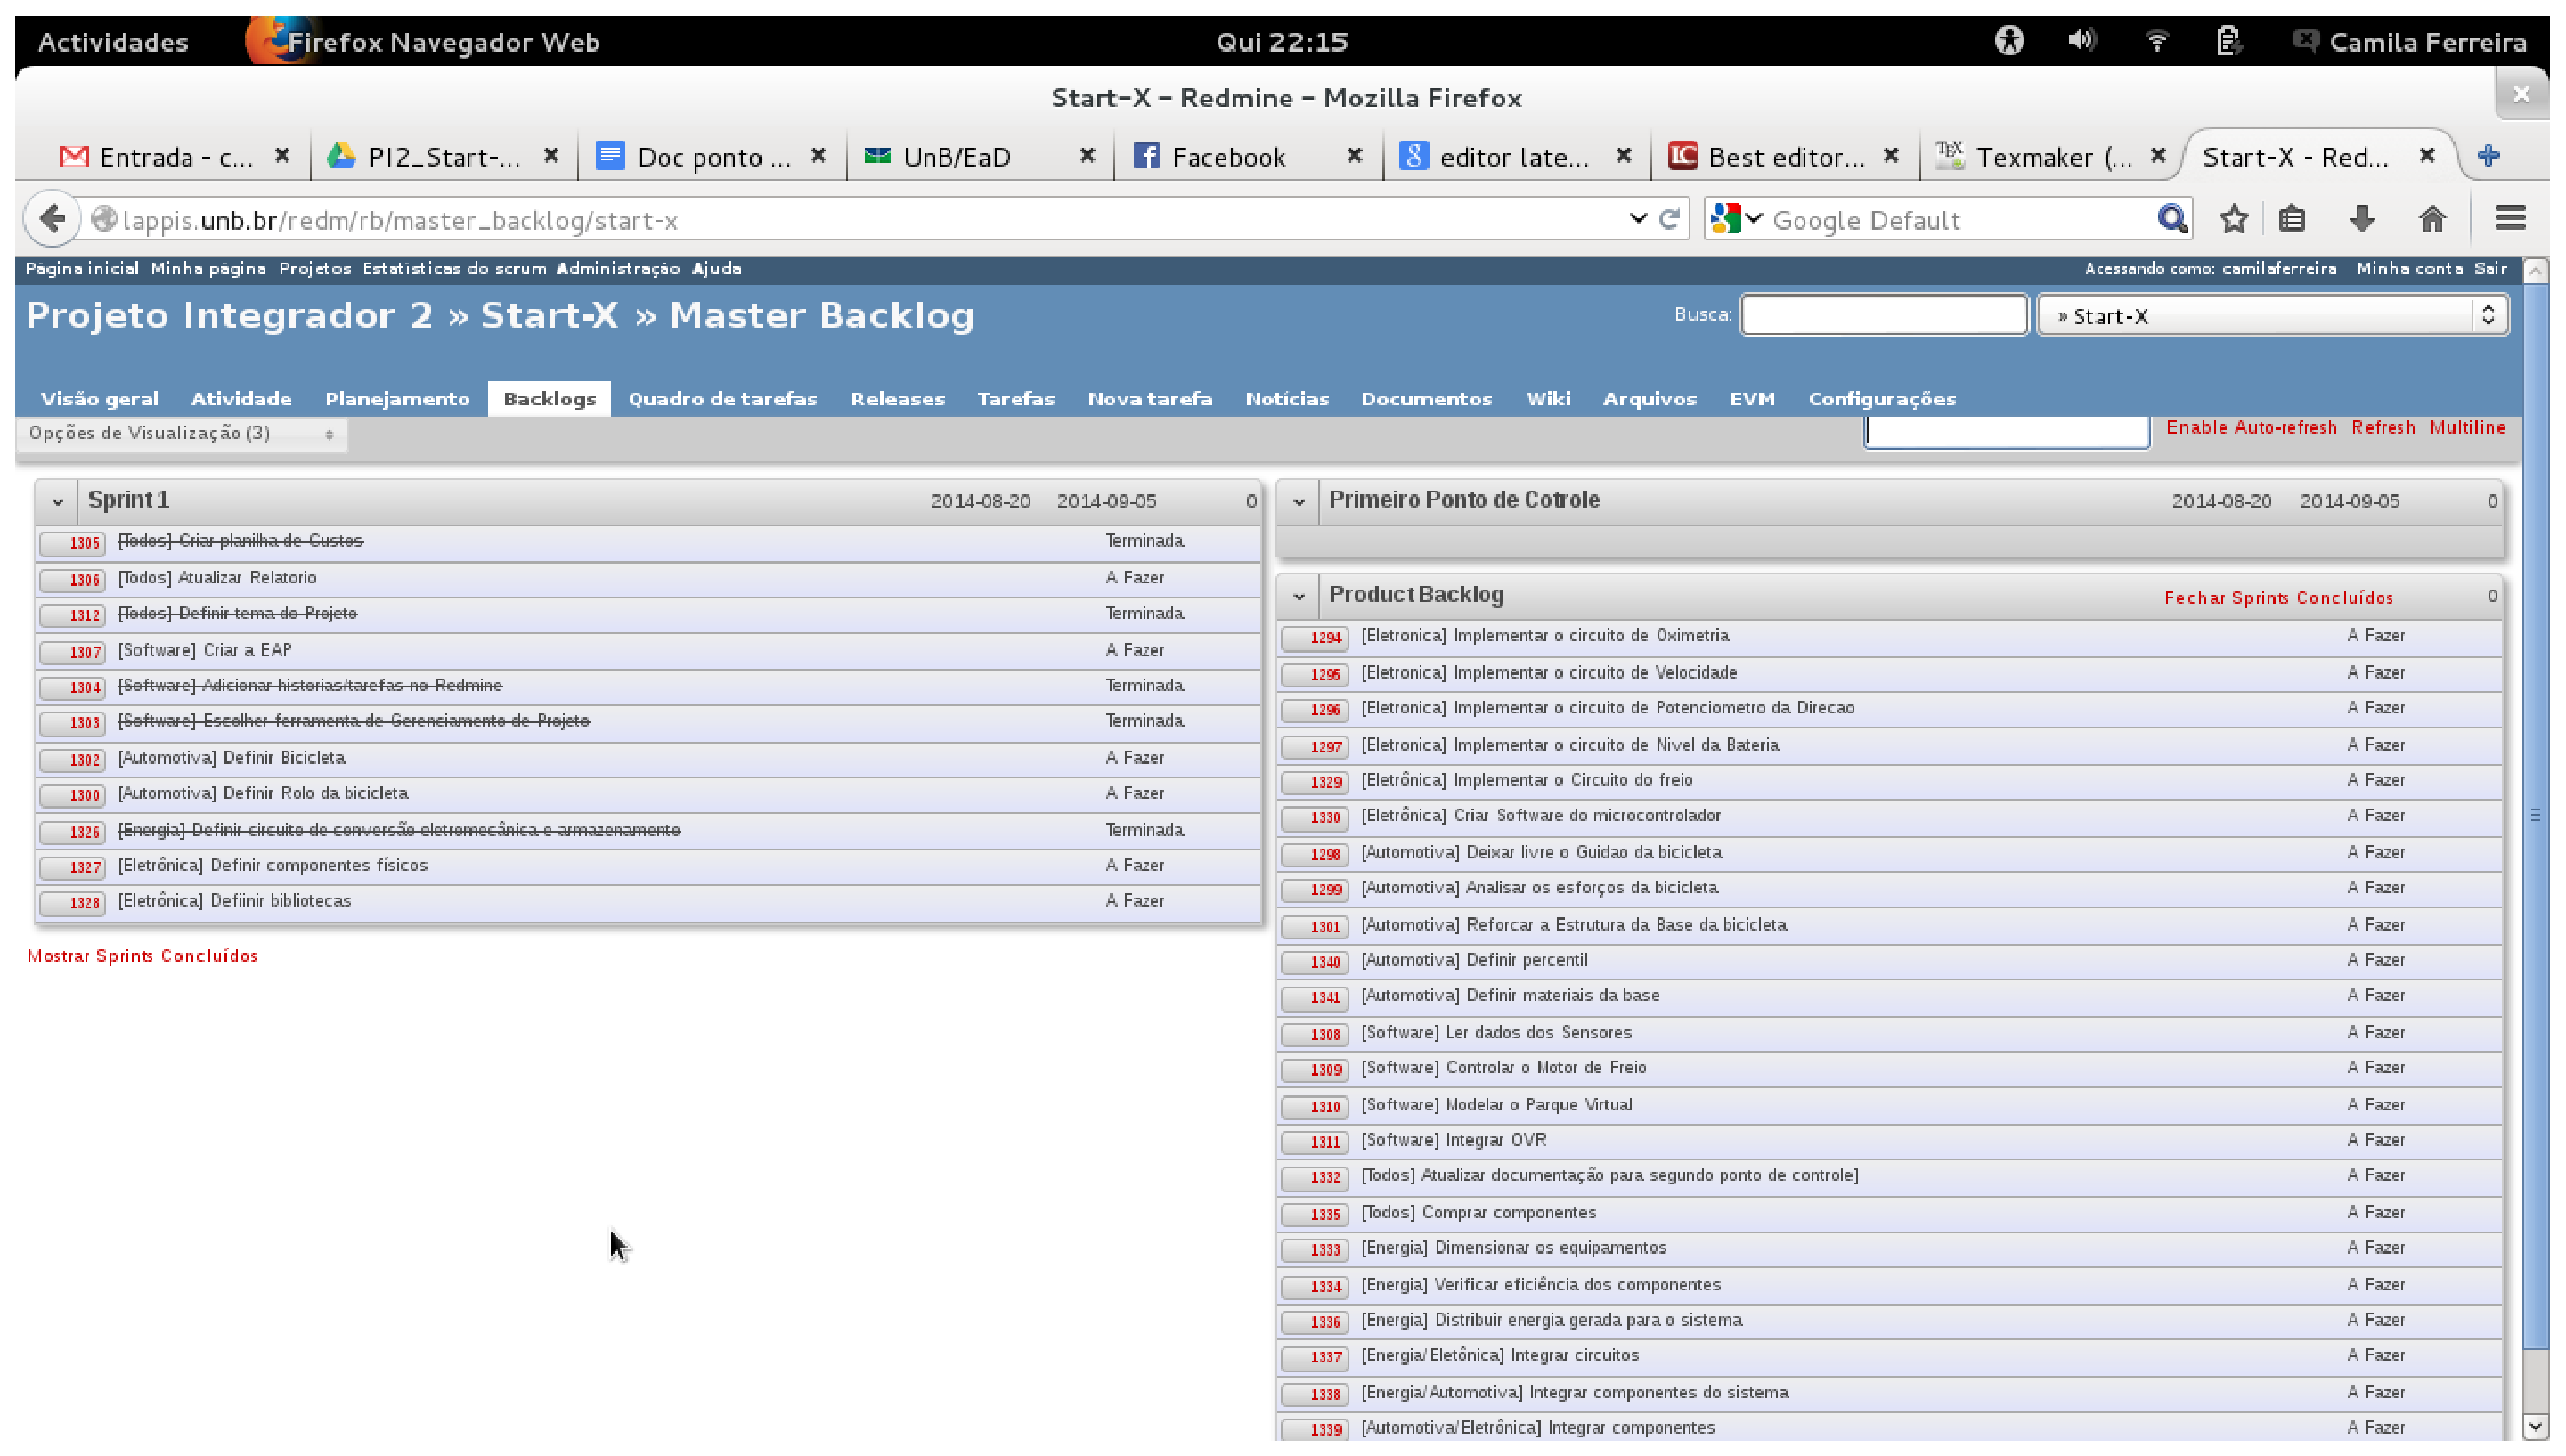
\includegraphics[width=0.7\textwidth]
      {figuras/backlogs.eps}
  \caption{Redmine e backlog do projeto}
  \label{redmine-backlog}
\end{figure}

\begin{figure}[h]
  \centering
  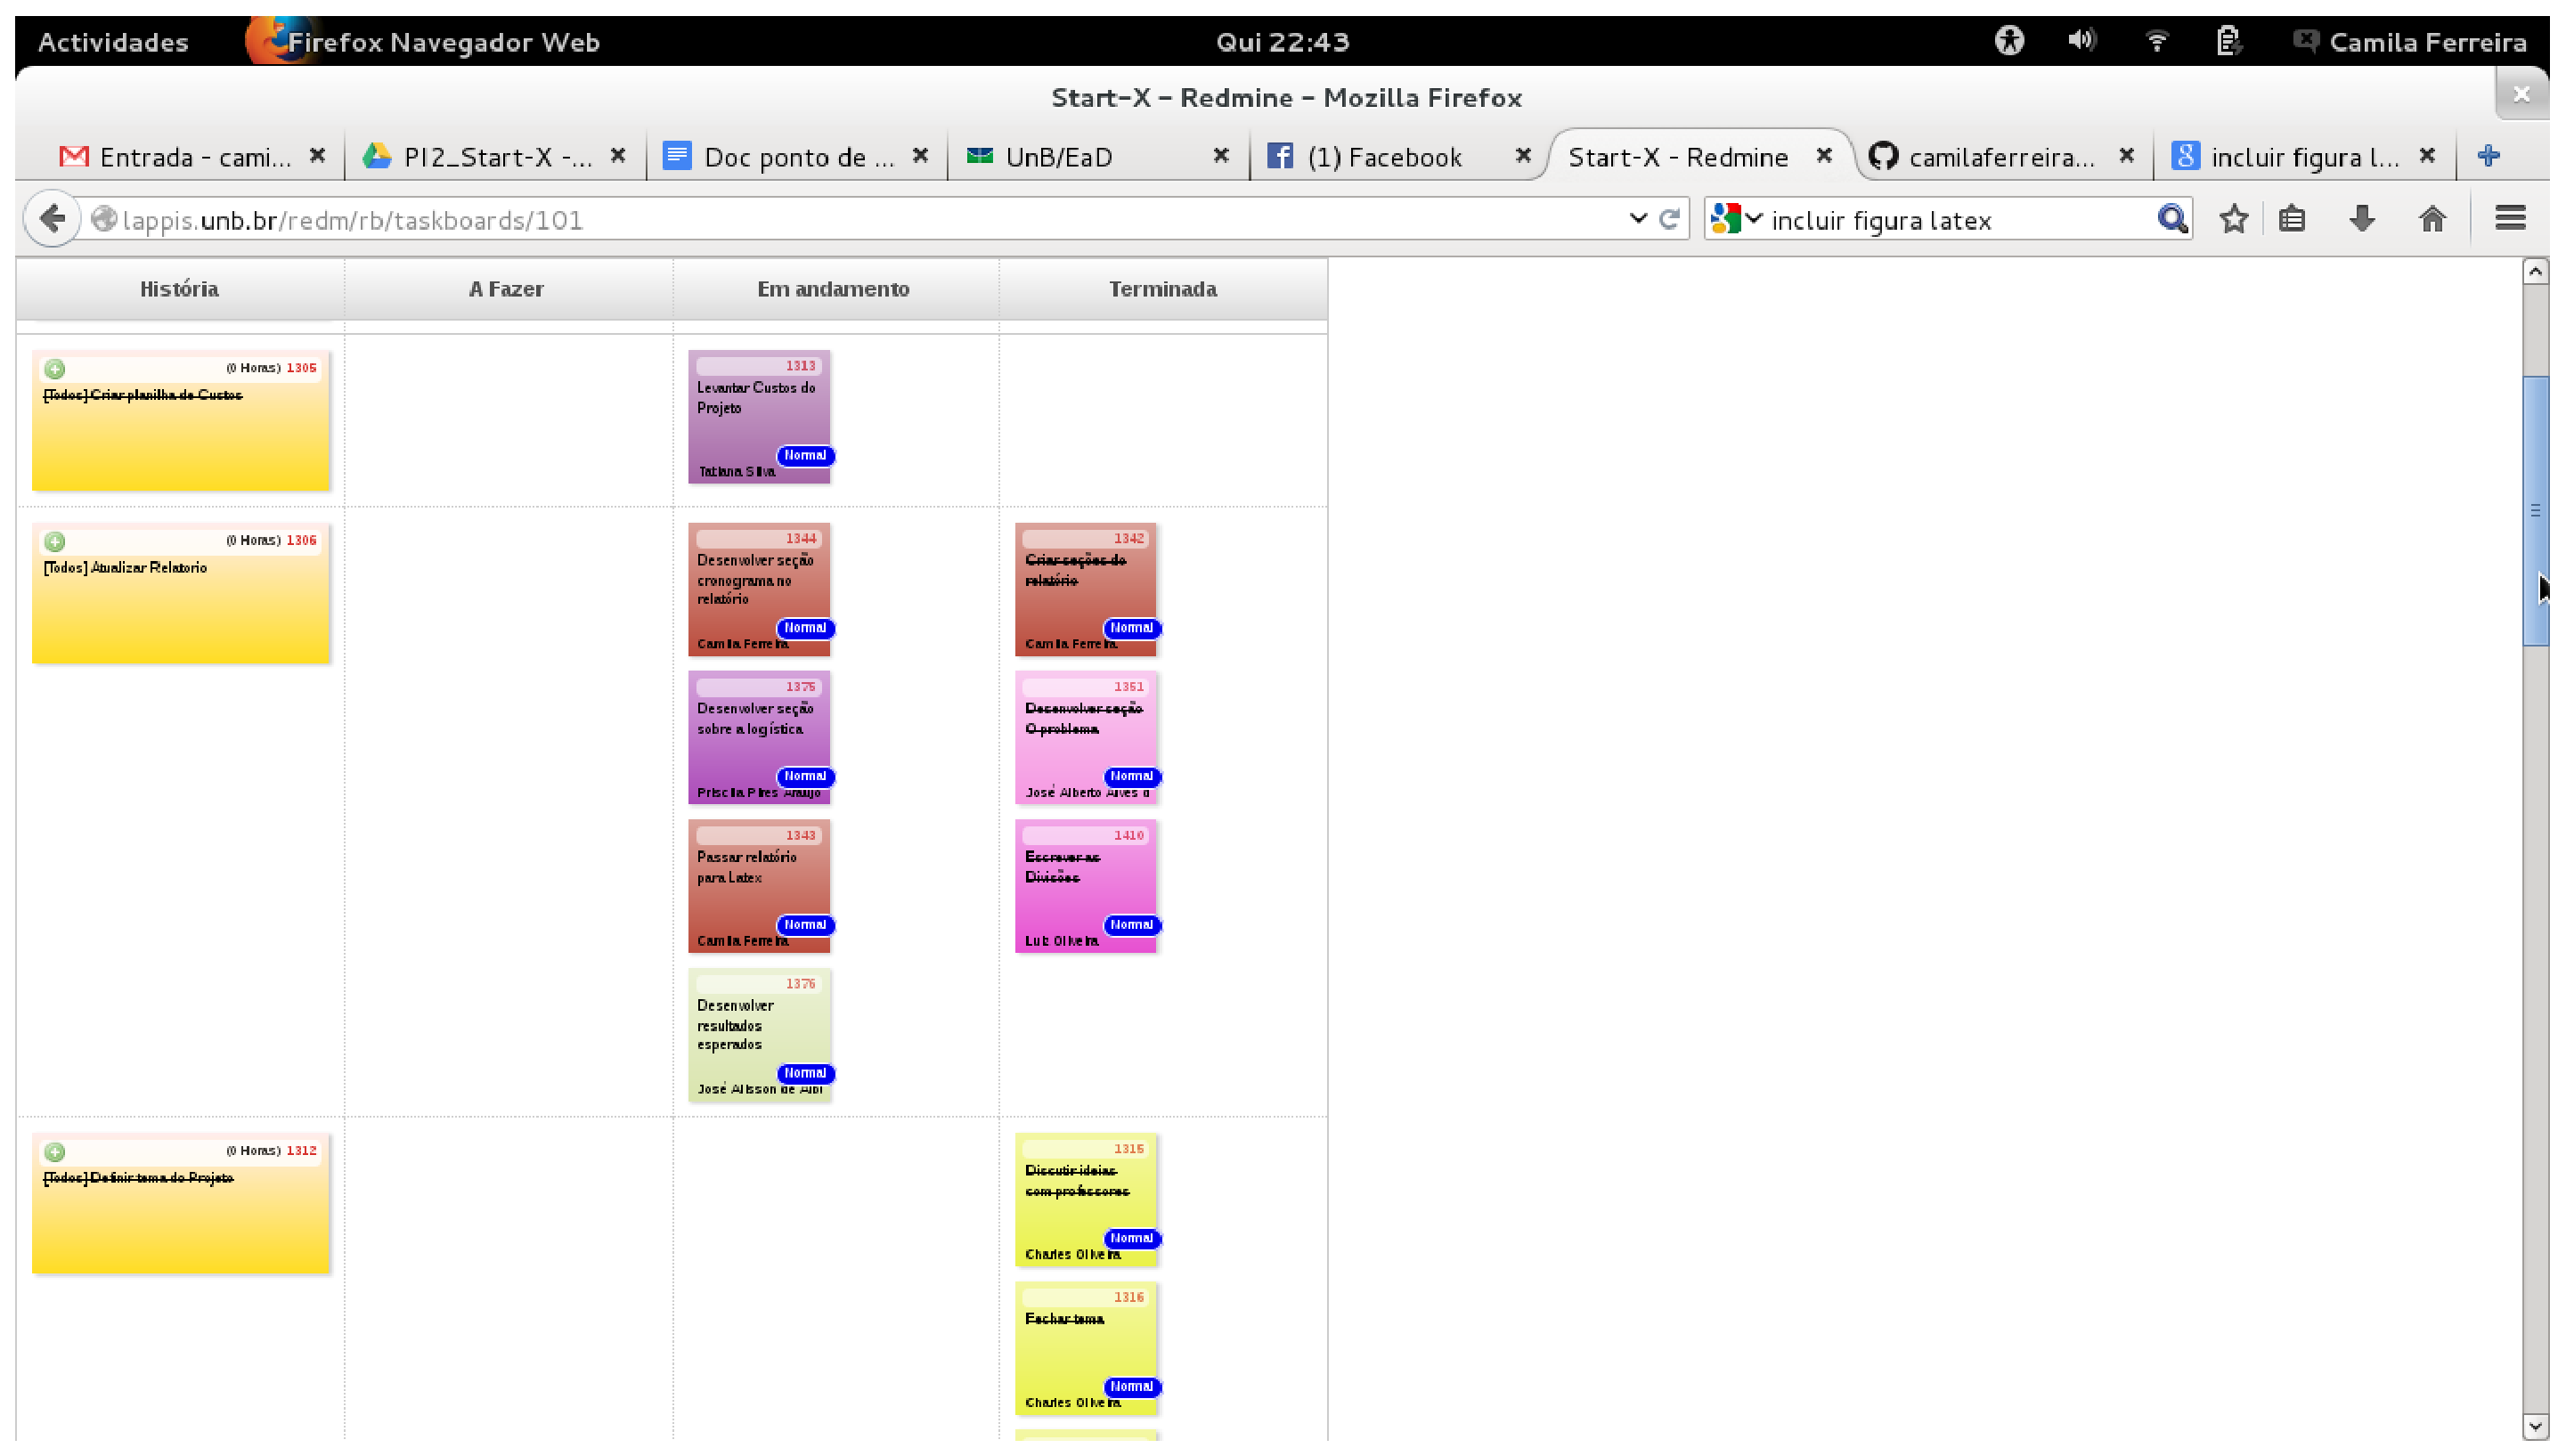
\includegraphics[width=0.7\textwidth]
      {figuras/quadrotarefas.eps}
  \caption{Quadro de tarefas}
  \label{quadro-de-tarefas}
\end{figure}
\newpage


\section{Cronograma}
Na figura quatro tem-se a Estrutura Analítica do Projeto - EAP, nela encontram-se os principais entregáveis do projeto. Com base nessa organização foi definido o seguinte cronograma para o projeto com três grandes pontos (datas a partir da Entrega 1 são aproximadas):
\begin{itemize}
  \item Entrega 1: 05/09/2014
    \begin{itemize}
      \item Viabilidade do projeto
    \end{itemize}
  \item Entrega 2: 31/10/2014
    \begin{itemize}
      \item Eng. Automotiva
        \begin{itemize}
          \item Ergonomia do produto
          \item Estrutura do produto
        \end{itemize}
      \item Eng. Eletrônica
        \begin{itemize}
          \item Montagem dos circuitos dos sensores
        \end{itemize}
      \item Eng. Energia
        \begin{itemize}
          \item Conversão eletromecânica
          \item Armazenamento de energia
          \item Eficiêcia energética
        \end{itemize}
      \item Eng. Software
        \begin{itemize}
          \item Modelagem do ambiente virtual
          \item Integração da modelagem
          \item Leitura dos dados dos sensores
        \end{itemize}
    \end{itemize}
  \item Entrega 3: 21/11/2014
    \begin{itemize}
      \item Energia/Software: Disponibilização dos dados de produção de energia
      \item Eletrônica/Software: Leitura dos sensores e informações no Oculus Rift
      \item Automotiva/Software: Acionamento dos freios em subidas virtuais
      \item Automotiva/Energia: Acoplamento da fonte motriz
      \item Eletrônica/Automotiva: Circuito que aciona os freios
      \item Eletrônica/Energia: Circuito controlador de energia produzida
    \end{itemize}
\end{itemize}
\begin{figure}[h]
  \centering
  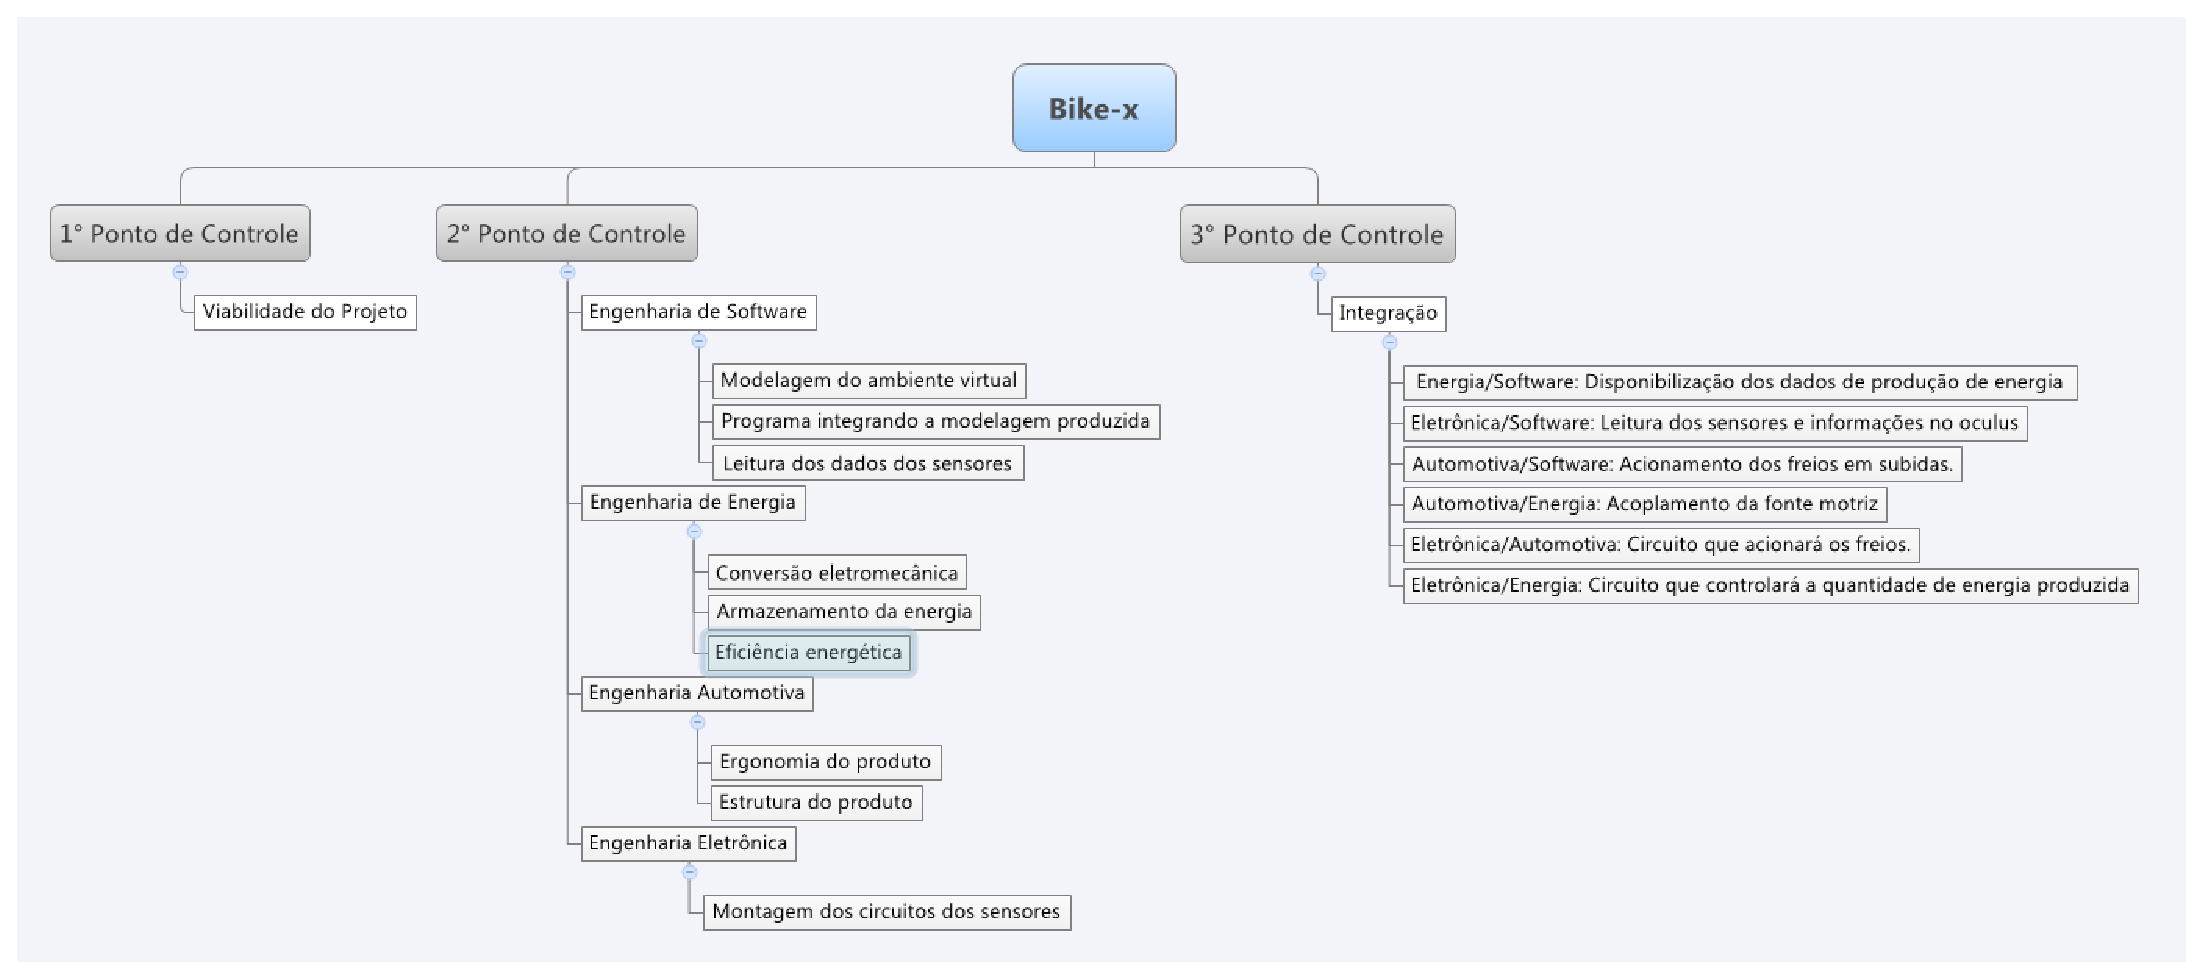
\includegraphics[width=1.2\textwidth, angle =90 ]
      {figuras/bike-x2.eps}
  \caption{EAP}
  \label{EAP}
\end{figure}




  
